\documentclass[10pt,a4paper]{article}
\usepackage[margin=20mm]{geometry}
\usepackage{amsmath,amssymb,graphicx,booktabs,microtype}
\usepackage[hidelinks]{hyperref}
\graphicspath{{results_L16/}}
\setlength{\parindent}{0pt}
\setlength{\parskip}{5pt}
\title{Redistribution, thermalization, and nonlinear gain\\in the large-$\ell$ QNM network}
\author{Numerical experiment summary}
\date{16 November 2026}
\begin{document}
\begin{center}
{\large\bfseries Redistribution, thermalization, and nonlinear gain\\
in the large-$\ell$ QNM network}\par
\small Numerical experiment summary --- 16 November 2026
\end{center}

\textbf{Main conclusion.}
The experiments distinguish conservative statistical relaxation from driven
coherent evolution with nonlinear gain and QNM loss. The closed kinetic system
transports action transiently and then reaches Rayleigh--Jeans (RJ) equilibrium.
The driven coherent system instead obeys an action balance whose outcome depends
on both the non-Hamiltonian interaction and the damping strength.
These are \emph{not} numerical demonstrations of coexisting stationary RJ and
Kolmogorov--Zakharov (KZ) regimes: no stationary constant-flux cascade is
established by these two figures.

\textbf{Setup.}
The examples retain the fundamental tower, with $\hat q=0.6$, $r_+=1$ and
$\alpha=1$. Coherent evolution is axisymmetric; kinetic occupations are
magnetically averaged, with degeneracy $g_\ell=2\ell+1$.
The displayed results use $\ell_{\max}=16$; consistency checks were also run at
$12$. Existing coefficient and evolution tools were left unchanged.

\section*{1. Conservative kinetic relaxation: transfer ends in detailed balance}
The first experiment solves $\partial_T n_\ell=\mathcal C_\ell[n]$, with
\emph{no forcing or damping}. Initial occupation is concentrated at
$2\le\ell\le4$, with a positive background and mean occupation normalized to one.
The conserved action and its finite-network RJ reference are
\begin{equation}
 N=\sum_\ell g_\ell n_\ell,\qquad
 n_\ell^{\rm RJ}=n_{\rm RJ}=\frac{N}{\sum_\ell g_\ell}=1.
\end{equation}
The constant occupation is appropriate to the exactly degenerate frequency
model: quadratic energy supplies no independent constraint here. Constant
occupation per mode does not mean constant action per shell; the latter is
$g_\ell n_{\rm RJ}$.

The diagnostics in Fig.~\ref{fig:kinetic} are
\begin{equation}
 \Pi(L,T)=-\sum_{\ell\le L}g_\ell\mathcal C_\ell[n],\qquad
 D_{\rm RJ}=\left[\frac{\sum_\ell g_\ell(n_\ell/n_{\rm RJ}-1)^2}
 {\sum_\ell g_\ell}\right]^{1/2}.
\end{equation}
Initially, action leaves the occupied band and populates higher shells; a
simultaneous low-shell component is visible in the signed flux. Subsequently
the spectrum flattens, the flux vanishes and $D_{\rm RJ}$ reaches the numerical
floor, approximately $6.4\times10^{-13}$. The entropy
$S=\sum_\ell g_\ell\log n_\ell$ increases up to roundoff-level fluctuations.
Thus early spectral transport and late RJ behavior are successive stages of
one conservative relaxation, not contradictory predictions.

An RJ state has vanishing quartet gain--loss brackets (detailed balance). A
stationary cascade would instead require a \emph{nonzero flux plateau} over
an interval between injection and removal. Transient flux or a spectral slope
alone does not establish that condition. This finite, closed experiment does
not test the existence of an extended forced KZ state.

\begin{figure}[!ht]
 \centering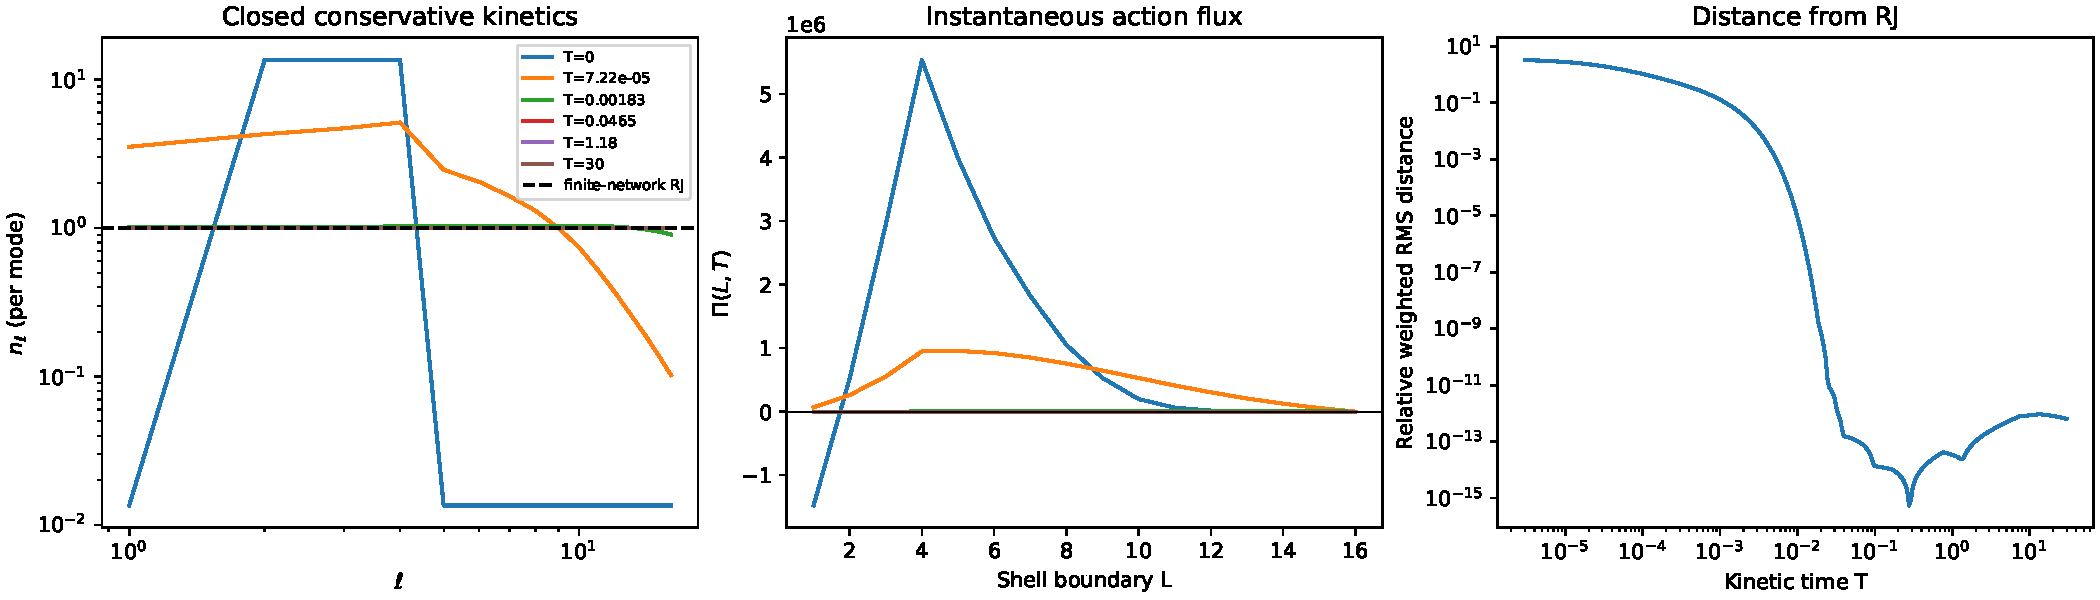
\includegraphics[width=\linewidth]{kinetic.pdf}
 \caption{Undamped, closed kinetic evolution: per-mode spectrum, instantaneous
 action flux and weighted distance from RJ. Late-time distances below roughly
 $10^{-12}$ reflect numerical error rather than resolved physical evolution.}
 \label{fig:kinetic}
\end{figure}

\clearpage
\section*{2. Driven coherent evolution: nonlinear gain versus QNM loss}
Here the low modes $\ell\le3$ are maintained as a unit-action pump, with
phase seed 7. The high band obeys the full cubic equations in slow time
$\tau=\epsilon^2t$, using
\begin{equation}
 C_\eta=C_H+\eta R,\qquad R=C-C_H,\qquad
 \partial_\tau A=-iF_H[a]-i\eta F_R[a]-\rho\gamma A,
 \quad\rho=\frac{\sigma}{\epsilon^2},\quad\gamma_\ell=\frac{h_\ell}{2}.
\end{equation}
Here $F_X[a]_\lambda=\sum_{ijk}X_{\lambda ijk}a_i a_j\bar a_k$ and
$a$ contains both the frozen pump and evolving high modes.
$C_H$ is the existing full Hamiltonian projection; $R$ is its residual.
The residual parameter probes the non-Hamiltonian interaction, rather than
an independently defined matrix anti-Hermitian projection.

The exact high-band action budget is
\begin{equation}\label{eq:budget}
 \frac{dN_{\rm h}}{d\tau}=J_H+G_R-L_{\rm QNM},\qquad
 G_R=2\eta\,\Im\sum_{\lambda\in{\rm h}}\bar A_\lambda F_R[a]_\lambda,
 \quad L_{\rm QNM}=2\rho\sum_{\lambda\in{\rm h}}\gamma_\lambda|A_\lambda|^2.
\end{equation}
$J_H$ is Hamiltonian exchange with the maintained pump; internal high-band
Hamiltonian interactions have zero total action contribution. Therefore
$N_{\rm h}$ can grow even at $\eta=0$. The residual term has no general sign
restriction, but supplies positive action in these examples. It is nonlinear
gain, not conservative transport. QNM loss is nonnegative and strengthens
with $\rho$ and, through $h_\ell\sim\ell+1$, with angular scale.

\begin{figure}[!ht]
 \centering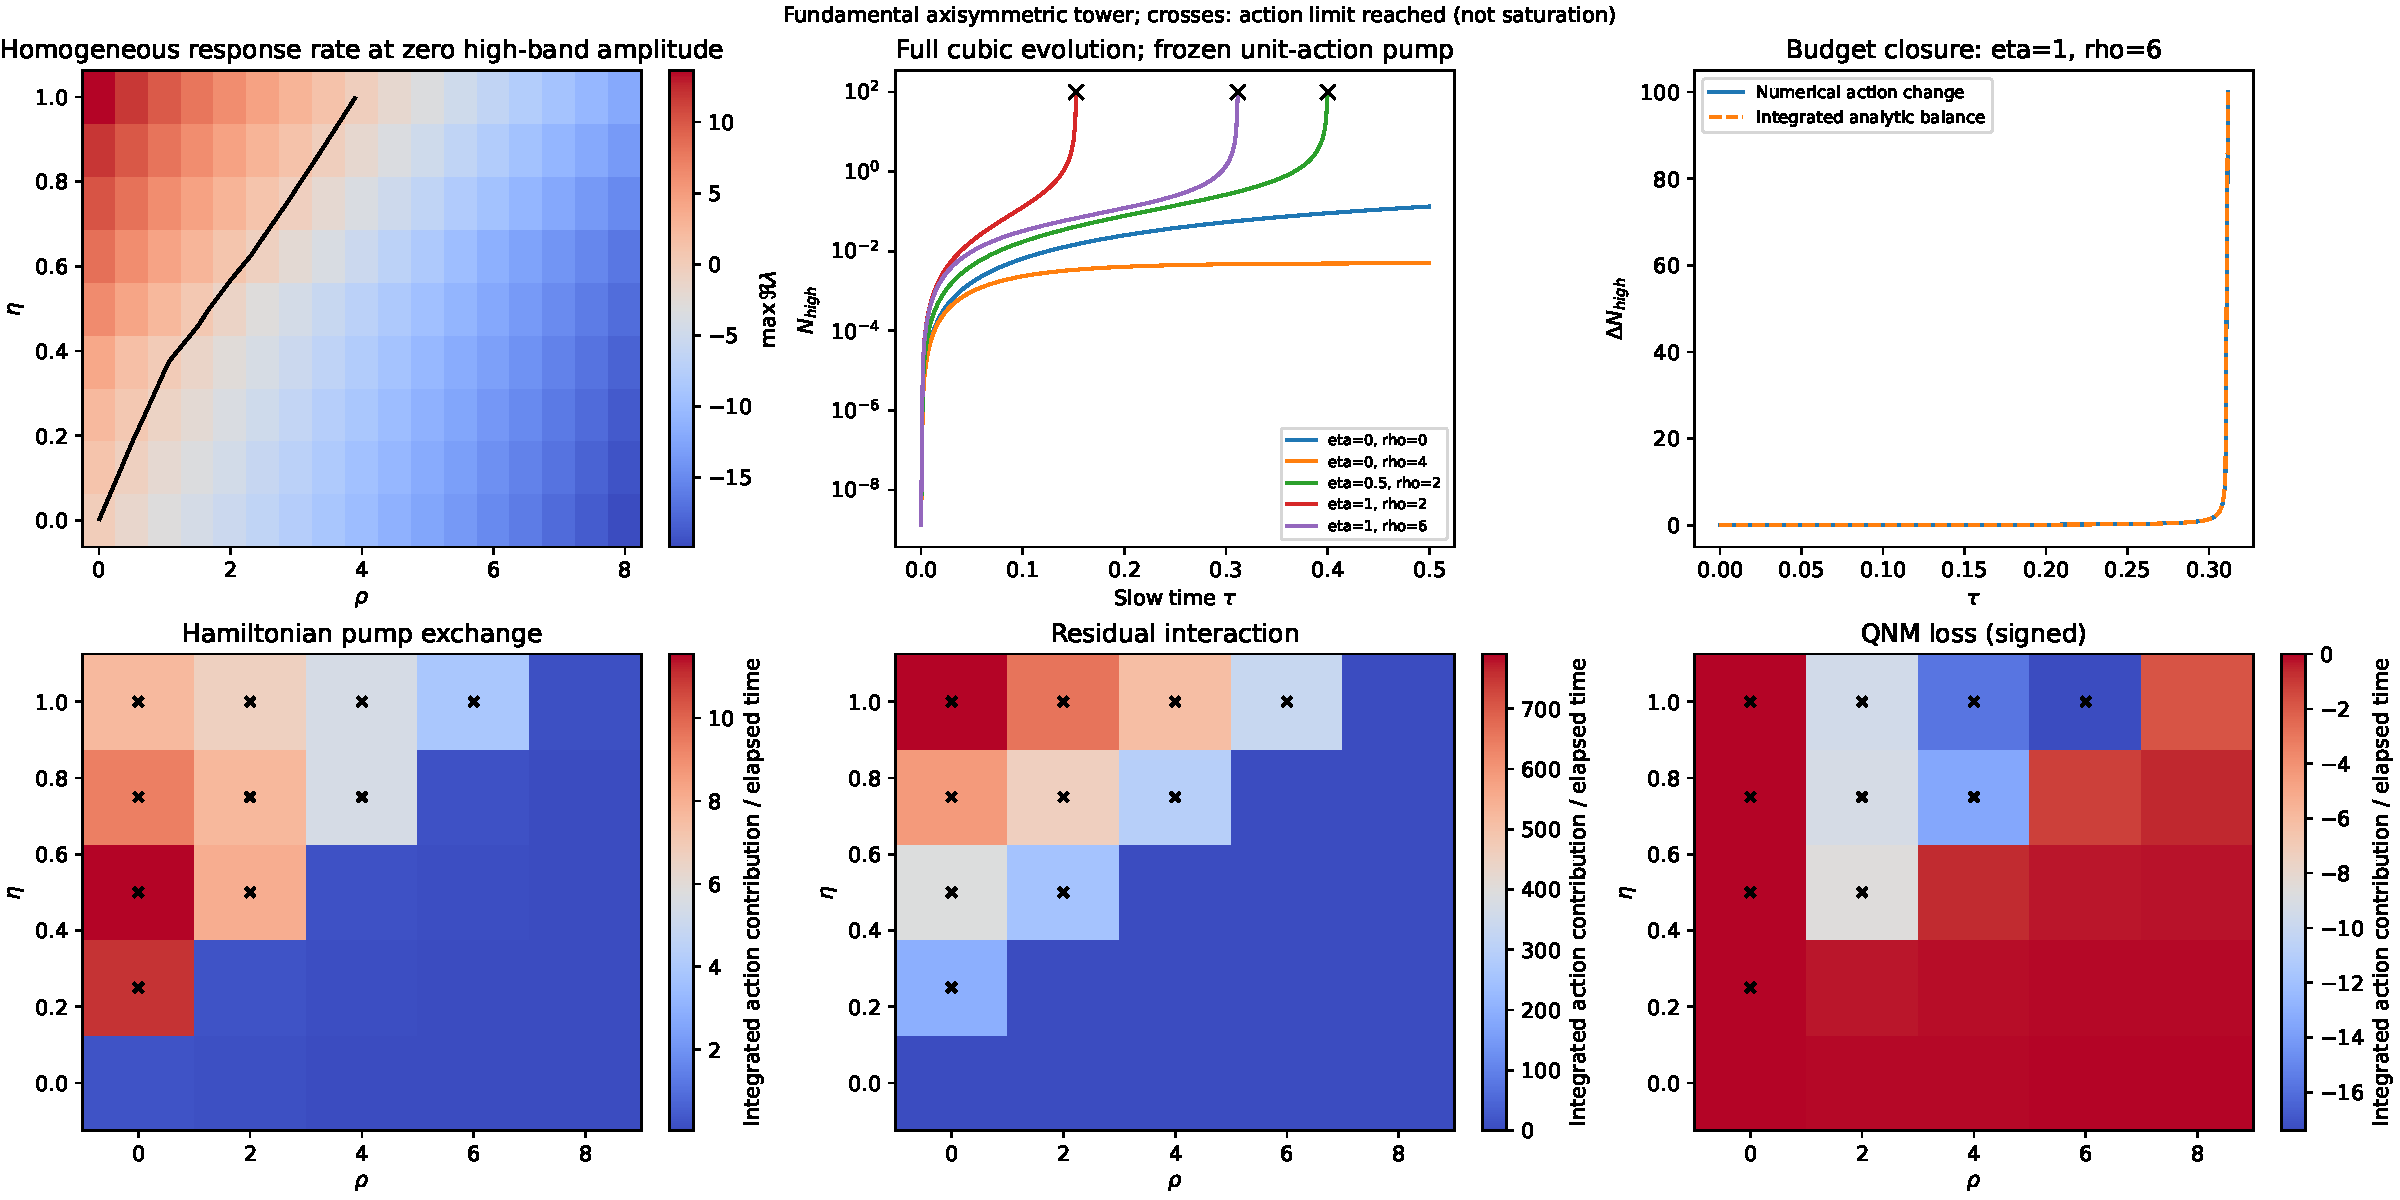
\includegraphics[width=\linewidth]{coherent.pdf}
 \caption{Coherent response and action balance. The upper-left panel is the
 homogeneous response at zero high-band amplitude; the lower panels are
 finite-time mean contributions to Eq.~\eqref{eq:budget}, with QNM loss shown
 with its negative sign. Crosses mark trajectories stopped at $N_{\rm h}=100$;
 their averaging durations differ. They are not saturated states.}
 \label{fig:coherent}
\end{figure}

Increasing damping clearly suppresses the Hamiltonian response: at $\eta=0$,
$N_{\rm h}(0.5)$ decreases from $0.1330$ at $\rho=0$ to $0.004981$ at
$\rho=4$ and $0.001312$ at $\rho=8$. For $\eta=1$, damping delays strong
growth: the action cap is reached at $\tau=0.1253$, $0.1999$ and $0.3117$
for $\rho=0,4,6$, respectively; at $\rho=8$, it is not reached by $0.5$,
when $N_{\rm h}=0.06291$. This last observation establishes only a bounded
response over the sampled interval, not long-time saturation.

\clearpage
\section*{3. What the linear threshold does, and does not, imply}
The response map uses the real-linear operator
\begin{equation}
 \delta\dot A=-i(\mathcal M\delta A+\mathcal P\delta\bar A)
                  -\rho\gamma\delta A.
\end{equation}
For $\eta=1$ its largest real eigenvalue crosses zero at
$\rho_c=3.9044003$, reproducing the notes' $3.904$. However, the pump also
produces an inhomogeneous source, so $A_{\rm h}=0$ is not a stationary solution
of the full problem. The response threshold is consequently not a global
nonlinear stability boundary.

At $(\eta,\rho)=(1,6)$ the zero-high-band response rate is $-6.3643$, yet
the forced cubic trajectory reaches the action cap. At increasing occupation,
the cubic interaction can overcome linear loss. A one-mode analogue makes the
sign and order explicit:
\begin{equation}
 i\dot A=(u+iv)|A|^2A-idA
 \quad\Longrightarrow\quad
 \dot n=2vn^2-2dn.
\end{equation}
Positive $v$ gives nonlinear gain, whereas $d>0$ gives linear loss. This
analogy explains a possible competition, not a fitted reduction of the full
network. The stopped trajectories prove neither physical runaway nor a
finite-time singularity. Large high-band action also requires reassessing the
frozen-pump and weakly nonlinear approximations. Stability of a forced
stationary state must be tested at that state.

\section*{4. Dissipation and the RJ--cascade distinction}
For a driven kinetic model,
$\partial_T n_\ell=\mathcal C_\ell+S_\ell-D_\ell n_\ell$, stationarity implies
\begin{equation}
 \Pi(L)=\sum_{\ell\le L}g_\ell(S_\ell-D_\ell n_\ell),\qquad
 \Pi(L+1)-\Pi(L)=-g_{L+1}D_{L+1}n_{L+1}
\end{equation}
above the forcing band. Distributed damping therefore consumes flux along
the band; a plateau requires losses to be negligible within the proposed
inertial interval. This balance explains how QNM damping can interrupt
transport, but the present undamped kinetic figure does not measure that
effect directly. A controlled kinetic damping sweep, including a boundary-only
sink for comparison, remains necessary to isolate it numerically.

Finally, coherent interaction and kinetic equilibration use different clocks:
$\tau=\epsilon^2t$ and $T\sim\epsilon^4t$ (with the existing kinetic prefactor
convention retained). The damping ratios scale as
$\rho=\sigma/\epsilon^2$ and $\rho_4=\sigma/\epsilon^4=\rho/\epsilon^2$.
Coherent coupling can thus develop while slower kinetic relaxation is
interrupted by decay. The two figures are separate controlled experiments,
not two trajectories at one specified physical $(\epsilon,\sigma)$.

\textbf{Verification and limits.}
Six tests check literal quartet contractions, action conservation, RJ
stationarity, the entropy-production square, gain/loss signs, the occupation
decay factor of two, pump scaling, Jacobians, matrix-exponential evolution,
and the reference threshold. At $\ell_{\max}=16$, relative kinetic action
drift is $9.4\times10^{-13}$ and the largest integrated coherent budget
residual is $4.6\times10^{-10}$. Tenfold tighter solver tolerances change
kinetic occupations by $3.8\times10^{-10}$ and selected coherent amplitudes
by at most $5.3\times10^{-9}$, relative to their respective amplitude scales.
The runs at $12$ and $16$ verify numerical consistency, not cutoff independence:
the kinetic initial total action changes with cutoff under mean-occupation
normalization. Raw data and checks are in
\texttt{results\_L12/} and \texttt{results\_L16/} beside this source.
\end{document}
